\documentclass[a4paper,10pt,twocolumn]{article}
\usepackage{amsmath}
\usepackage{graphicx}
\usepackage{newtxtext,newtxmath}
\usepackage{lipsum}
\usepackage{tabularx}
\usepackage{booktabs}
\usepackage{algorithm}
\usepackage{algorithmic}
\usepackage{float}
\usepackage{geometry}
\usepackage{draftwatermark}
\usepackage{titling}
\usepackage{makeidx}
\usepackage{url}
\SetWatermarkText{DRAFT}
\SetWatermarkScale{1}
\geometry{
a4paper,
total={170mm,257mm},
left=20mm,
top=20mm,
}

\frenchspacing

\pretitle{%
\begin{center}
\LARGE

\includegraphics[width=50mm]{logo-min}\\[\bigskipamount]
}
\posttitle{
	\normalsize
	\end{center}}



\title{Aidos Kuneen \\ --- A Blockless and Anonymous Cryptocurrency for the Post-Quantum Era ---}

\author{
	Aidos Developer \and Aidos Foundation
}
\date{December XX, 2017 \\ Version 0.035.\\ THIS IS A DRAFT. THIS LINE MUST BE INCLUDED IN TRANSLATIONS.}


\begin{document}

\twocolumn[
	\maketitle

\begin{abstract}
		In this white paper we introduce a new cryptocurrency, \emph{Aidos Kuneen}. Aidos Kuneen has been developed to deliver a 
		fast, anonymous, blockless, decentralized and scalable solution for post-quantum era transfers with zero fees. 
		
		Aidos Kuneen employs a mechanism known as \emph{iMesh}, within iMesh all transactions are directly referenced by
		one another in order to form a \emph{Directed Acyclic Graph (DAG)} structure.
		
		The inclusion of `SPECTRE' allows full-nodes to determine which transactions are legitimate within the DAG structure and
		to reject those that are not. In addition, SPECTRE provides resilience against any attackers who may control up to 50\% 
		of the network's computational power.
		
		To ensure continued security in the post-quantum era, Aidos Kuneen utilises the hash-based signature `XMSS'. XMSS
		provides for both a small signature and small public key size which in turn reduces network load.
	
		In order to provide anonymity within the network, Aidos Kuneen employs \emph{AKShuffle}. AKShuffle 	
		incorporates the post-quantum, Zero-knowledge proof `ZKBoo (ZKB++)`, this allows for truly anonymous transfers 
		throughout the entire network.
		
		To allow Aidos Kuneen to service the expected growth of the future `IoT' sector we introduce a cooperative Proof of Work
		mechanism known as \emph{coPoW}. coPoW allows a number of senders within the network to co-operatively perform the 
		necessary Proof of Work in order to confirm the transactions on the network, thus reducing the physical processing 
		requirements of any one sender.
		
		Finally, we provide a simulation of the number of leaves in iMesh and we further determine the minimum number of 
		reference transactions required in order to converge the DAG and deliver faster confirmation times for transactions 
		while having minimum effect on the transaction size.
		
		\end{abstract}

		\vspace{0.5cm}

Copyright \copyright 2017-2018 by Aidos Developer and Aidos Foundation. \\

IN NO EVENT SHALL THE AUTHORS OR COPYRIGHT HOLDERS BE LIABLE FOR ANY CLAIM, DAMAGES OR OTHER
LIABILITY, WHETHER IN AN ACTION OF CONTRACT, TORT OR OTHERWISE, ARISING FROM,
OUT OF OR IN CONNECTION WITH THE WHITEPAPER OR THE USE OR OTHER DEALINGS IN
THE WHITEPAPER. \\

This work is licensed under a Creative Commons Attribution 4.0 International License. \\
\url{http://creativecommons.org/licenses/by/4.0/} \\

\includegraphics{cc}
]

\twocolumn[
\tableofcontents
]

\clearpage

\section{Introduction}
Bitcoin, the once obscure cryptocurrency introduced by Satoshi Nakamoto~\cite{btc} in 2008, has now begun to draw much wider attention 
from both the general public and governments alike. Within the Bitcoin network, transactions are written into `blocks', these blocks are 
then crypographically validated by powerful computers known as `miners' using a Proof of Work (PoW) system. Once a block has been 
validated it is then appended to a continually extending chain known as the `block-chain'. Miners are subsequently rewarded for 
sucessfully validating a block by means of the transaction fees paid by senders who transact on the Bitcoin network. Currently, blocks 
are added to the blockchain at a rate of approximately one every 10 minutes. The transactions consist of both input and output 
addresses, with the inputs themselves being the outputs of previous transactions, this provides an auditable history of all past Bitcoin 
transactions within the network. In order to prove ownership, transactions are signed by the address owner with an Elliptic Curve 
Digital Signature Algorithm (ECDSA).

However, in recent years a number of problems have been identified with the Bitcoin implementation, including:
\vspace{-0.5\baselineskip}
\begin{itemize}
	\setlength\itemsep{0em}
	\item{Limited scalability}\mbox{}\\ 
	Within the core Bitcoin code, the maximum block size is restricted and blocks are unable to store transactions once this limit 
	is exceeded. This in turn leads to a scalability problem when many transactions are broadcast simultaneously with many of them 
	being unable to be included in the current block.
	\item{High fees}\mbox{}\\ 
	Senders are required to pay a transaction fee in order to incentivise the miners to include their transaction in a block.
	If Bitcoin usage continues to grow and the price of Bitcoin increases, the relative value of the fee will also increase. At some
	point it will no longer make sense to send small transactions via the Bitcoin network and the fee would be greater than the 
	value of the Bitcoin being transacted. This forces senders to use complicated schemes to send small value trasnactions (e.g. 
	micropayment channels).
	\item{Weak cryptographic strength for quantum computers}\mbox{}\\ 
	As of 2017, the development of quantum computers is still in its infancy. However, experiments have already been carried out in 
	which quantum computational operations were executed on a small number of quantum bits. Furthermore, Google has reported its 
	intent to commercialize quantum technologies within the next five years~\cite{google}.At the same time, according to Shor's 
	algorithm~\cite{shor}, all algorithms based on the elliptic-curve discrete logarithm problem (including ECDSA as used in 
	Bitcoin), can be easily solved with a sufficiently powerful quantum computer. 
	\item{Weak anonymity}\mbox{}\\ 
	The auditable nature of Bitcoin means that in order to spend Bitcoin, the spending transaction must refer back to the founding
	transactions that came before it, these founding transactions are open to the public. As such, anyone is free to track the flow
	of btc from address to address.
\end{itemize}

We introduce a new cryptocurrency, \emph{Aidos Kuneen} in order to address these problems.
Aidos Kuneen is based on \emph{Directed Acyclic Graph (DAG)} technology known as \emph{iMesh}.
In iMesh, transactions are directly referred to by other transactions and as such, there are no blocks and no block-chain.
The confirmation of a transaction are determined by the number of other transactions which \emph{vote}
for the transaction based on the DAG structure. In iMesh, we are able to achieve the benefits of scalability while removing the 
requirements for mining incentives in the form of transaction fees.

\vspace{-0.5\baselineskip}
\begin{itemize}
	\setlength\itemsep{0em}
	\item{More scalable}\mbox{}\\ 
In iMesh, one performs relatively easy PoW to confirm the transaction. After the transaction is broadcast to the network, the 
transaction is stored into iMesh immediately. Hence there is no need to wait for one's own transaction to be stored. Additionally 
there is no limitation to the size or number of transactions tha can be stored at a time. The more iMesh grows, the more transactions 
become involved. This means that the confirmation time of any single transaction will reduce.

\item{No fee}\mbox{}\\ 
One does not need to pay any fees, because there are no miners. No fee means one is free to transaction any amount, no matter how small 
without requiring any special techniques.

\item{Post quantum computers}\mbox{}\\ 
In Aidos Kuneen we employ hash-based signature which has strong post-quantum security instead of ECDSA.
There are many signatures for post-quantum, including Ring-LWE based, Lattice based and hash-based signature.
However most of them are not practical due to the key size or the signature size.
The key size of Ring-LWE and Lattice based signature are around a few Kilo Bytes. This means, for example, that we 
must copy and paste a long string on the website to let people know his address. This is not practical for normal use of cryptocurrency.
One of hash-based signatures, e.g. SPHINCS, by which we can use the public key many times, also suffice from the public key size (about 1 KByte).
We decided to use eXtended Merkle Signature Scheme (XMSS). By XMSS we can use a same public key for a certain times (e.g. 1000 times or can be more).
The size of public key is 32 bytes and signature key size is about 3 KBytes.
Also these has 128 bits post-quantum security, which is sufficient for long-term secure post-quantum system~\cite{recom}.

\item{Strong anonymity}\mbox{}\\ 
For anonymity, we utilize post quantum zero-knowledge non-interactive(ZKNI) proof `ZKBoo' mentioned in~\cite{zkboo}.
One sends coins to an address which is an output of encryption, and spends the coin without revealing her secret key.
\end{itemize}

\section{Related Works}

For anonymity Monero\footnote{http://monero.org/} and ByteCoin\footnote{https://bytecoin.org/} use `ring signature'
mentioned in CryptoNote~\cite{ringsig}.
Ring signature relies on signature which has a trapdoor function (e.g.\ public key encryption), but unfortunately hash-based signature
doesn't have the feature.  Zcoin\footnote{https://zcoin.io/} uses zero-knowledge non-interactive proof called zk-SNARKs, but zk-SNARKs is  not
post quantum, because it uses pairing-based cryptography as Zcoin developers are discussing\footnote{post-quantum Zcash (https://github.com/zcash/zcash/issues/805)}.
As mentioned in the discussion we don't see any pairing-based crypt for post quantum.

Another option for anonymity is to use CoinJoin or its variants (e.g. CoinShuffle). But CoinJoin
requires participants at the same time one wants to send tokens. This could be critical while there
are few users for Aidos Kuneen.
Instead,  Aidos Kuneen uses `ZKBoo' as ZKNI  scheme which uses only hash and encryption which are secure for quantum computers.

We talk about two differences with IOTA\footnote{https://iota.org/}, which is also DAG-based cryptocurrency without fee,  

First, they are using ternary based signature instead of binary based one. This is  because theoretically urinary is more efficient than binary.
We use traditional binary based signature to fully utilize existing CPU features 
(SIMD instructions and dedicated SHA extensions etc).because we strong believe recent digital processors are well fast and efficient, and
some of processors for IoT already have dedicated circuits for SHA-2 based hash, e.g.~ARM processors\footnote{https://static.docs.arm.com/ddi0501/f/DDI0501.pdf}.
And we use XMSS so that we can sign more than one time by one address.
Additionally we introduce the scheme for doing PoW cooperatively with many senders for IoT devices.

Second, IOTA is claiming that network would corrupts if there are \( 2/3 \) of malicious nodes. But if we follow IOTA's
confirmation process in their whitepaper one counts only number of referring transaction (descendant transactions). Intuitively we notice that
if there are many leaves in DAG  (it can occur normally),  number of descendant transactions  of one transaction would be small.
Then attackers could  grow their malicious transactions faster than the network. 
Instead, we introduce the confirmation process based on \emph{SPECTRE} mentioned in~\cite{spectre}.
In SPECTRE  one doesn't only counts the number of  descendant transaction,
but also counts number of other transactions which vote the transaction. 
Hence even if the leaves diverge, it's hard for attacker to grow confirmations of their malicious transactions.

In SPECTRE voting process, we still need faster DAG convergence for faster confirmations.
IOTA white paper doesn't clarify the convergence.
(The whitepaper is saying `One \emph{expects} that the \( L(t) \) (total number of leaves) remains stable.')
Therefore we additionally simulate the behavior of leaves in iMesh to ensure that DAG converge earlier.

\section{Signature Scheme}
\label{sec:sig}

We use XMSS and its parameters described in RFC draft of IETF~\cite{ietf}.
XMSS is based on Winternitz One Time Signature (WOTS+). 

WOTS+ is a hash based signature scheme for one time use.
And XMSS is a technique to make it possible to sign messages more than two times with one key.

\subsection{WOTS+}

\begin{figure}[ht]
	\begin{center}
	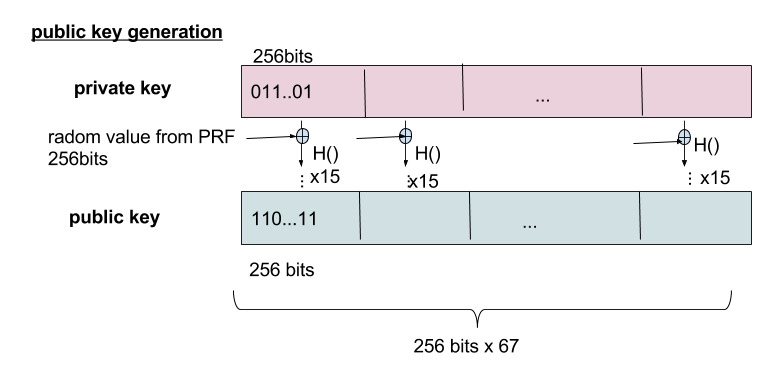
\includegraphics[width=80mm]{wots_pub.png}
	  \caption{Generation of WOTS+ public key}
    \label{fig:wots_pub}
	\end{center}
 \end{figure}

 Figure~\ref{fig:wots_pub} explains how to generate a public key.

 To generate a public key, one gets 67 number of 32 bytes (256 bits) random binary data as his private key \( Priv_{j}, j=1 \ldots 67\).
 Then each \( Priv_{j} \) are hashed with SHA-256 for 15 times. While hashing, each  \( Priv_{j} \) is XORed with a value from PRF (Pseudo Random Function).
 This XOR operation is a trick to reduce the signature size with same security level.
 Finally he gets 67 number of 32 bytes binary data. This is his public key \( Pub_{j}, j=1 \ldots 67\).

 \begin{figure}[ht]
	\begin{center}
	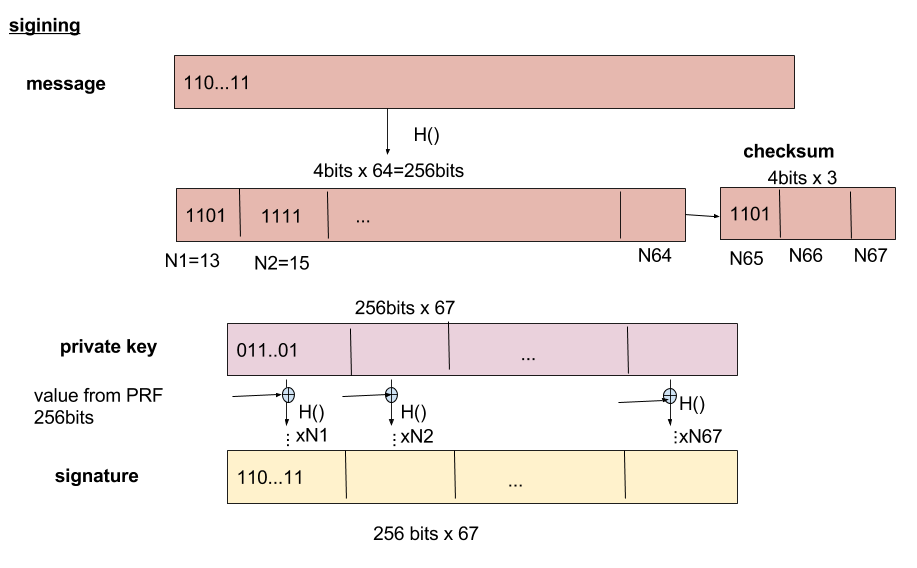
\includegraphics[width=80mm]{wots_sign.png}
	  \caption{Signing with WOTS+ private key}
    \label{fig:wots_sign}
	\end{center}
 \end{figure}

 Figure~\ref{fig:wots_sign} shows  how to sign a message.

 For signing one gets 256 bits hash of his message, and calculates a 12bits checksum from the hashed message.
 Then he gets 4 bits 67 binary data from the message.
 These values are shown as \(N_i,i=1 \ldots 67\) in the figure. Each 4 bits binary of \( Priv_j \) are hashed for
 \(N_i\)  times after XORed with same values he used for \( Pub_{j} \). 
 This result \( Sig_j, j=1 \ldots 67 \) are the signature.
 This checksum is used for preventing attacks from malicious messages. For example, if an attacker make a message  whose hash is 000 \ldots 0,
 i.e. \( N_i = 0, i=1 \ldots 64 \), then the signature completely would equal to his private key if there is no checksum. 

 \begin{figure}[ht]
	\begin{center}
	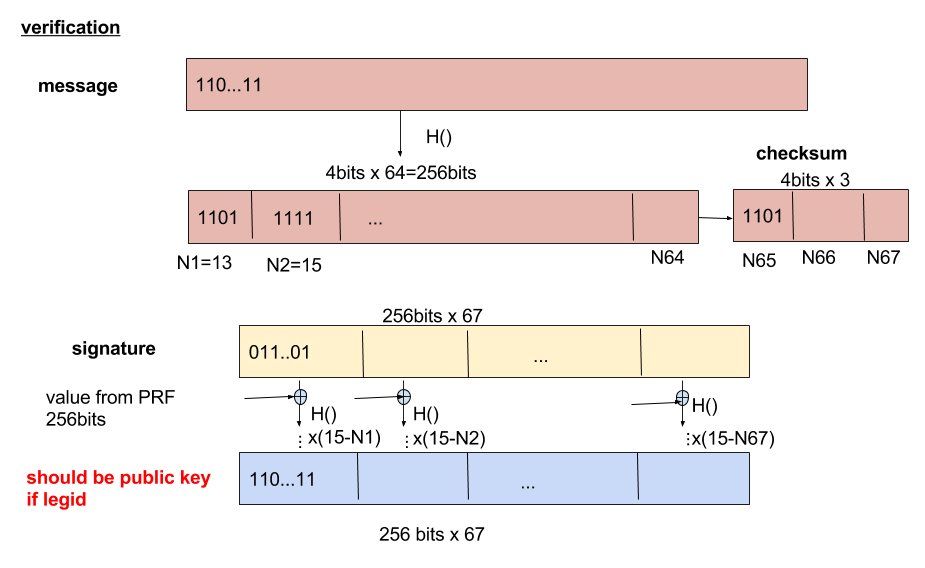
\includegraphics[width=80mm]{wots_veri.png}
	  \caption{WOTS+ Verification }
    \label{fig:wots_veri}
	\end{center}
 \end{figure}

 Figure~\ref{fig:wots_veri} shows  how to verify a signature.

 For verification a verifier calculates \(N_i, i=1 \ldots 67 \) in the same way as signing explained above.
 Then each \( Sig_j \) are hashed for \(15-N_i\)  times after XORed with same  values  used for \( Pub_{j} \).
 He gets \( Pub'_j , j=1 \ldots 67\). Then he checks if  \( Pub'_j,  j=1 \ldots 67 \) equals singer's public key \( Pub_j,  j=1 \ldots 67 \).

\subsection{XMSS}

\begin{figure}[ht]
	\begin{center}
	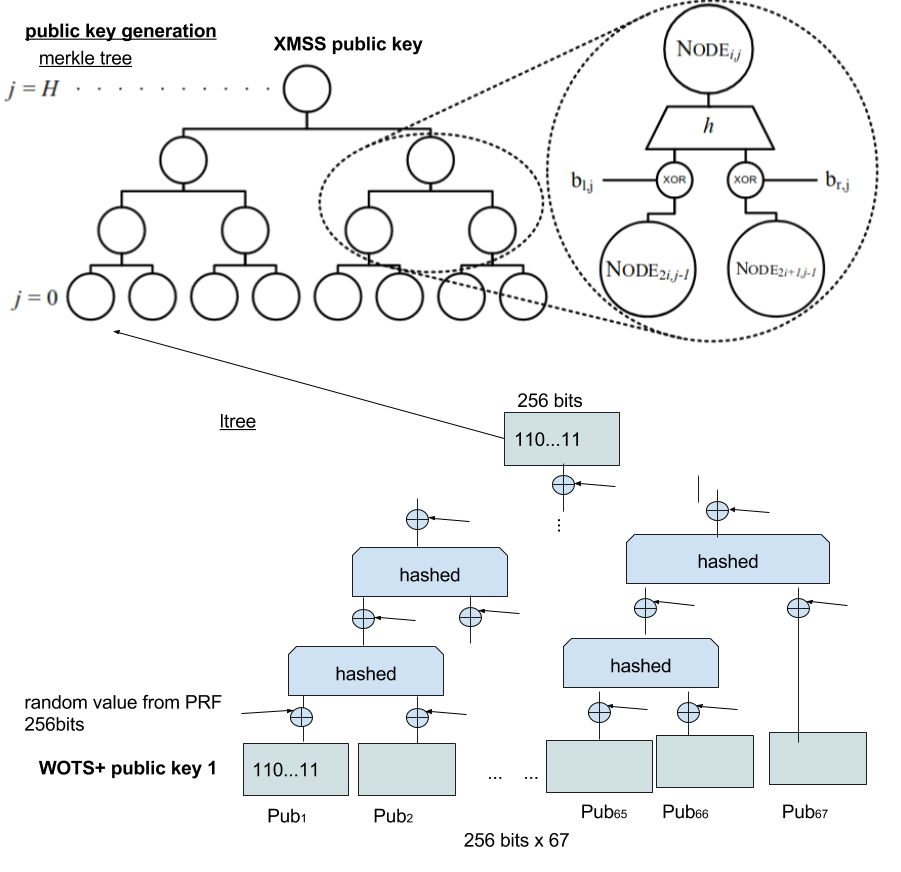
\includegraphics[width=80mm]{xmss_pub.png}
	  \caption{Key generation}
    \label{fig:xmss_pub}
	\end{center}
 \end{figure}

Figure~\ref{fig:xmss_pub} shows how to generate a public key for XMSS. In short XMSS builds a tree called Merkle Tree
to gather all public keys into one public key. Therefore one can use one public key for many times.

At first one must make \( 2^h \)  numbers of WOTS+ private keys \( Priv_{ij}, i = 1 \ldots 2^h ,  j=1 \ldots 67\) and 
corresponding WOTS+ public keys \( Pub_{ij}, i = 1 \ldots 2^h , j=1 \ldots 67 \)  (\(h\):height of Merkle Tree).
We denote \( Pub_{ij} , j=1 \ldots 67 \) as  \( Pub_{i} \).
Then  `ltree's are made
from each public keys. One gets root hash of the ltree by hashing together with sibling WOTS+ public key
( e.g.  \( Pub_{i} \) and  \( Pub_{i+1} \) ) repeatedly. This root hash is one of leaf
in Merkle Tree.
So he repeats it to make \( 2^h \) number of ltrees to fill all leaves of Merkle Tree.
Finally, he gets the root hash of Merkle Tree by hashing leaves of the Merkle Tree (i.e. roots of ltrees).
The root hash is the public key of XMSS.

For signing, one selects one of unused private keys and corresponding public key.
And he calculates WOTS+ signature. XMSS signature is the WOTS+ signature with `auth path'. Auth path is additional
binary data to calculate root hash of Merkle Tree (i.e. XMSS public key).

\begin{figure}[ht]
	\begin{center}
	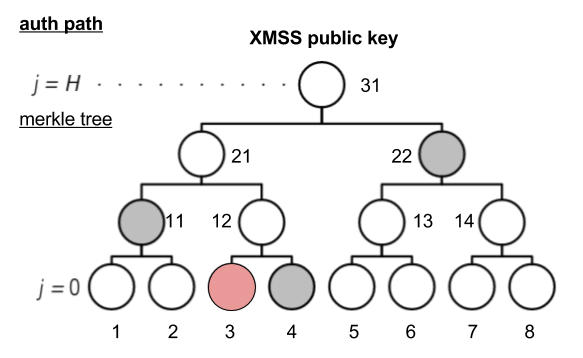
\includegraphics[width=80mm]{auth_path.png}
	  \caption{Auth path for XMSS}
    \label{fig:xmss_auth}
	\end{center}
 \end{figure}

In Figure\ref{fig:xmss_auth}, we assume 
to select No.3 private key for signing. A Verifier can calculate No.3 node from signer's signature. The Verifier need No.4 to get No.12.
, so auth path includes No4. In the same manner, to get No.31 root hash (i.e. XMSS public key), the signer includes  No4, No11 and No22 as auth path.

For verification, a verifier must get WOTS+ signature and node values on auth path.
She can calculate root hash of Merkle Tree, hence sh can  check if
the root hash equals to the XMSS public key.

Notice that
\vspace{-0.5\baselineskip}
\begin{itemize}
	\setlength\itemsep{0em}
	\item Signers need to record which private keys are used. We use Logarithmic Merkle Tree Traversal scheme 
	mentioned in \cite{traverse} for efficient traversal and least storage cost.
	\item Public key consists with \(32 \times 2 \) bytes (root hash of Merkle Tree and seed of PRF).
	There is only one PRF seed because all pseudo random values can be generated from one PRF.
	We include the seed as a part of a signature so that public key size becomes 32 bytes.
	\item  Signature key size is about 3 KBytes.
	\item Hash (SHA-256) has strong preimage resistance (i.e.\ attacker cannot guess the input from an output of hash),
	 so it's hard to guess private keys from public keys even if they use good quantum computers.
\end{itemize}
		
Additionally notice that we can use the same public key more time
if \(h\) (height of Merkle Tree) is increased more, but it takes time to generate public keys on initial stage.
Therefore in Aidos Kuneen there are 3 types of height.

\begin{table}[ht]
	\caption{Merkle Tree height, estimated time for key generation per one CPU core, and users of XMSS}
    \label{tbl:height}
	\begin{tabular}{rrrl} 
		\toprule
		height  & \#keys & key generation & user \\ 
		\midrule
			  10 & 1,024 &  a few seconds & one time user  and\\
			  & & & normal user \\
			  16 & 65,536 & a few minutes & companies\\
			  20 & 1,048,576 & \( \approx \) 30 minutes &  big companies\\ 
			  \bottomrule
			\end{tabular}
  \end{table}

Table~\ref{tbl:height} shows these 3 types. Those who wants to change addresses
per one payment or don't send coins over 1000 times  
could use height=10 without less impact of generating public keys. Big users, e.g.
companies or merchants, who do payment many times with one public key, would use height=16 or 20.

Note that we won't use XMSS \(^{MT}\) mentioned in~\cite{ietf}. 
Although XMSS \(^{MT}\) make us possible not to generate all public keys at once,
signature size is much bigger than XMSS (around 40 KBytes).


\section{iMesh}
\label{sec:imesh}

\subsection{SPECTRE}
When a sender sends a transaction \(T\),  he directly includes some previous transactions \(T\) which were sent before by others. 
Figure~\ref{fig:imesh} shows the DAG structure of these transactions we call \emph{iMesh}. When sending
the sender selects some leaves in DAG (i.e.\ transactions which are not referred by any transactions) he saw in iMesh.

\begin{figure}[ht]
	\begin{center}
	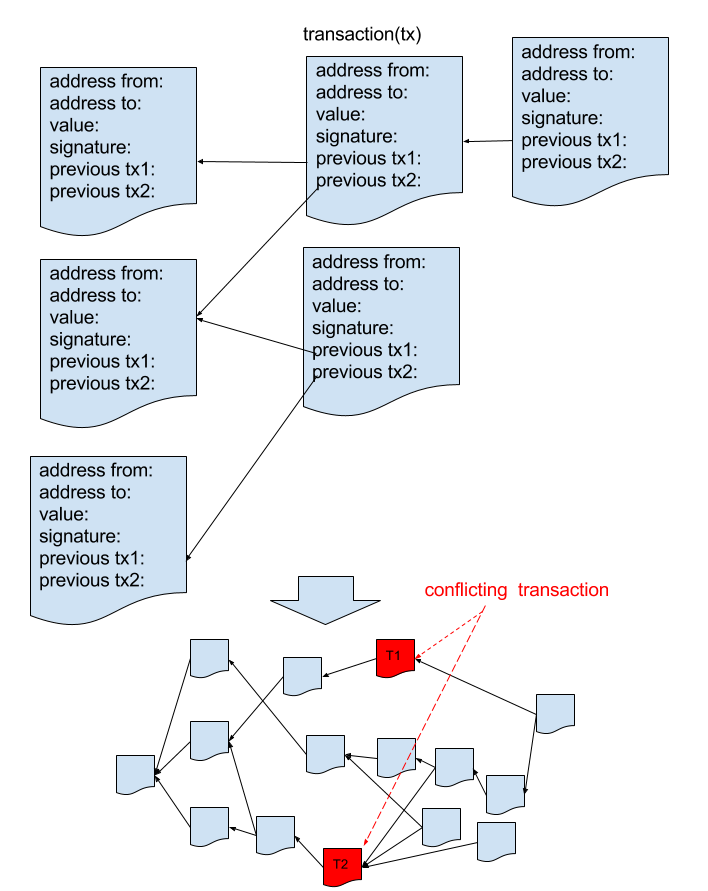
\includegraphics[width=65mm]{dag.png}
	  \caption{iMesh}
    \label{fig:imesh}
	\end{center}
 \end{figure}

Although blocks in Bitcoin refers one previous block,
DAG can refer many transactions in one transaction.
 Blocks grow one block per one time, but many transactions in DAG can grow simultaneously.
So, DAG can be more scalable than block-chain.

However there is a side-effect when there are conflict transactions.
For example, assume address Alice has 10 unit of coins.
She sends 10 units to Bob in transaction T1, and Alice sends 10 units to Cathy
in another transaction T2. As a result these 2 transactions are conflicting.
In block-chain based cryptocurrency, once one of them is stored in one block, another will be never stored,
i.e. if T1 is once confirmed,  T2 will be never validated.
On the other hand  when there are conflicting transactions (colored with red in Figure\ref{fig:imesh}) in iMesh,
it is hard to know which is valid. To solve this problem, we use voting mechanism  mentioned in `SPECTRE'~\cite{spectre}.
Note that any attackers cannot try anything but `double spending' attack mentioned above,
because nobody can create coins \emph{out of thin air}.

\begin{figure}[ht]
	\begin{center}
	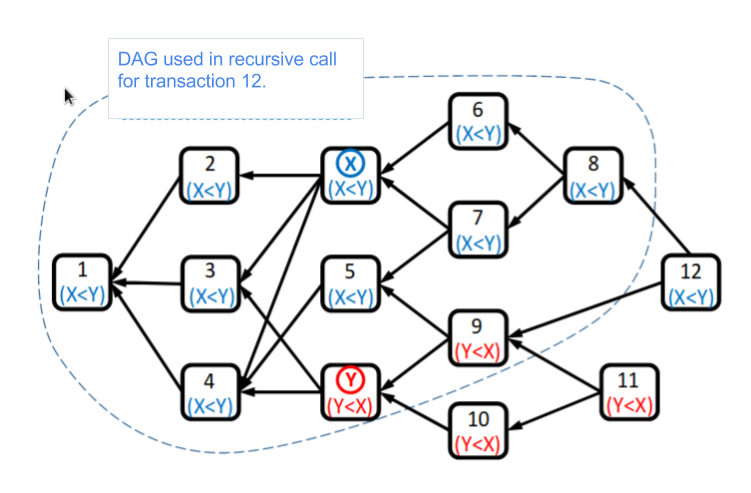
\includegraphics[width=80mm]{spectre.png}
	  \caption{An example of the voting procedure  on  a  simple  DAG.}
    \label{fig:spectre}
	\end{center}
 \end{figure}

 In SPECTRE one counts voters for conflicting transactions.
 Figure~\ref{fig:spectre} shows the voting procedure. 
 
 In this figure transaction x and y are conflicting.
 Transaction x and transactions 6--8 vote transaction x, as they only see x in their past, and not y. Similarly, transaction y and transactions 9--11 vote y.
 Transaction 12 votes according to a majority of votes of transactions except transactions 10,11,12. Any transaction from 1--5 votes x,
 because it sees more x voters in its future than y voters. As a result, x voters are more than y voters, x is regarded as legit. 

 Intuitively,  the procedure of voting and its reasons is as follows.

 \vspace{-0.5\baselineskip}
 \begin{enumerate}
	 \setlength\itemsep{0em}
\item   Transactions which only have the transaction x as parent vote transaction x. (transaction 6--8 and 9--11) \\
Honest transactions gain votes over withheld transactions in secret, as honest nodes keep adding new transactions to the honest transaction.
 \item  Transactions which have both x and y as parent vote to one of them which has majority of voters. (transaction 12)\\
 It guarantees majority amplification, as these transactions add votes
 that comply with and enhance previous decisions. 
 \item   Transactions which doesn't have both transactions x and y as parent vote to one of them which has majority of voters. (transaction 1--5)\\
 This rule allows amplifications in parents of x (transaction 1--4) to vote in its favour against y.
 This is needed to counter a pre-mining attack scheme, i.e. the attacker builds blocks and withholding them from the network.
 This is because honest transactions tends to have more ancestor transactions, and the honest transaction
 should get more votes by procedure 1 and 2.
 \end{enumerate}

Note that SPECTRE is resilient to attackers with up to 50\% of the computational power, and not 33\%, as is proved in~\cite{spectre}.

 Also in iMesh receivers must wait for their transaction to be confirmed by sufficient number of transactions like Bitcoin.
~\cite{spectre}  also mentions about how long receivers should wait. Let's assume that we wait 5 confirmations for Bitcoin 
and attackers in Bitcoin have 30\% of whole hash power. The possibility of success in attack is 17.8\%\cite{btc}. In SPECTRE voting scheme
one transaction needs around 130 referred transactions to get 17.8\%. 
If arrival of transactions becomes faster in iMesh , the waiting time would be shorter. But she would have to wait for a long time
in early days of iMesh. Additionally when an attacker has more than half of the whole hash power, the iMesh could be attacked
and malicious transactions could be illegally accepted.
Therefore we introduce a mechanism called `Coordinator` to confirm transactions deterministic ally for early days of iMesh.
Another thing we must note that if there are many leaves in iMesh, the possibility which one leaf is referred by one new transaction
would be less. So we need to consider how many number of transactions should be referred from one transaction. We will discuss this problem
in Section~\ref{sec:leaves}.

In voting scheme, senders have incentive to refer as many as transactions they can.
It's because the confirmation speed of senders' transaction also depends on the number of referring transactions.
So if a sender refers just few transactions, the receiver could reject the payment because it would take time to receive coins.

\subsection{Coordinator}

As mentioned previous section, we must assume that attackers could get half of PoW power in early days of
iMesh. This would make attackers to have big incentive to attack iMesh. Having half of PoW means that
we could not use automatic consensus. Thus we introduce `Coordinator' which 
confirms transactions by centralized way.

Each nodes define one trusted address (Coordinator) and  transactions which the trusted transaction refers are regarded as `confirmed'.
Rules to decide valid transactions between conflicting transactions are as follows.

\begin{itemize}
	\item  The transaction which is confirmed earlier is valid, and others are invalid.
	\item If  conflicting transactions are confirmed at same time,
	the transaction which has older time stamp is valid.
	If both of them has same time stamp, the transaction which has smaller hash
	is valid.
\end{itemize}

Trusted transactions must refer previous one to define `time stamp' in iMesh.
Each full nodes check the rule for each trusted transaction.
Coordinator is regarded as invalid if it doesn't refer previous transaction or refers older one.
It makes the Coordinator not to be able to try double spending.

Some people might say that the Coordinator is a centralized scheme and should not exist
in cryptocurrency. The Coordinator
is needed due to no fee and there is less incentive to contribute iMesh
in early days of iMesh. We strongly believe that no fee is a big advantage
for users. And don't forget that the Coordinator is not a main stream 
and it could be removed after the users  increase as mentioned before.

\section{Proof of Work}
\label{sec:pow}

When sending transactions, senders must do Proof of Work (PoW) as miners do in Bitcoin.
Each transactions have nonce field
and the hash of the transaction must be under certain value.  The time of PoW would be targeted
around 5--10 minutes in average.
PoW in Aidos Kuneen is for protecting DDoS and double spending attack to iMesh. 

Additionally PoW can disperse the distribution
of transactions occurrence. So we could re-target the difficulty of PoW when iMesh will be bigger.

We use Cuckoo Cycle mentioned in \cite{cuckoo} as PoW. The reason is as follows.
There would be much more transactions than blocks in Bitcoin, and full-nodes
must check PoW for all transactions. Therefor full-nodes would verify
PoW function much more time than Bitcoin. So we should not use heavy-weight PoW function (e.g.\ cryptonight or scrypt).
On the other hand ASICs and FPGAs should not be effective for PoW.
So we select Cuckoo Cycle, which  uses a few hundreds MBytes of memory.
PoW time is dominated mainly by  memory access speed, so ASICs and FPGAs are not effective.
Also it is much more light-weight to verify the PoW than cryptonight or scrypt.

We will use parameters:

\begin{itemize}
	\item \(cycle = 20\) to minimize the size impact to transactions.
    \item number of nodes = \( 2^{25} \). Memory usage should be around 128MB.
    \item \(easiness = 100\% \) to prevent optimizations e.g. by edge trimming.
\end{itemize}

\section{Cooperative Proof of Work}
\label{sec:copow}

For IoTs, whose performance is low, we introduce cooperative Proof of Work called \emph{coPoW}.
By coPoW, each senders can do PoW together with one transaction in which  senders' transactions are mixed up.
By coPoW we can utilize the IoT feature which the number of them is enormous.

coPoW acts like a mining pool in Bitcoin in decentralized manner:

\vspace{-0.5\baselineskip}
\begin{enumerate}
	\setlength\itemsep{0em}
	\item One who wants to join coPoW broadcasts a request to network via full-node.
	\item Others who also want to join coPoW or are already doing coPoW response its request.
	\item He joins to the coPoW group
	\item He does leader selection, or he gets who is the leader.
	\item He sends his transaction to the leader and gets mixed transactions from the leader.
	\item He starts PoW.
	\item He periodically sends result of PoW to the leader.
	\item He periodically receives PoW result of other parties from the leader. 
	\item If any of their results are incorrect he leaves the group.
	\item The leader rejects members who don't send their results in a certain period or send incorrect result. In this case the leader
	sends a restart command to members.
	\item Once he receives a result which matches to the final target, he finishes coPoW.
\end{enumerate}

Parties in a coPoW group must send their result (nonce of transaction) periodically whose hash 
is easier than the final target (\emph{target for proof}). This prevents free riders, who joined the coPoW but actually doesn't do PoW.
Target for proof could be variable. For example, target for proof = final target \(  \times 2^5 \) could be for groups for IoT devices,
target for proof = final target  \( \times 2^2 \) could be for groups for normal PCs.

Members in a group could use Tor for anonymity.


\section{AKShuffle}
\label{sec:aks}

For anonymity we use \emph{AKShuffle}. In AKShuffle, we utilize zero-knowledge non-interactive (ZKNI) proof for
anonymous payment. By ZKNI one can proof that her value satisfies some functions without revealing her secret key.
For example Alice has input \(x\)  and key \( k \)  for an encryption function \( f_{k}(x) \) and shows \( y=f_k(x) \) to Bob.
Bob wants to know Alice really has \(k\), but Alice doesn't want to reveal her \(k\).
By ZKNI  she can prove she really has \( k\).

We utilize ZKBoo (ZKB++) mentioned in~\cite{zkb} for ZKNI. ZKBoo uses only a hash and an encryption function (AES) which are quantum-safe.


\begin{figure}[ht]
	\begin{center}
	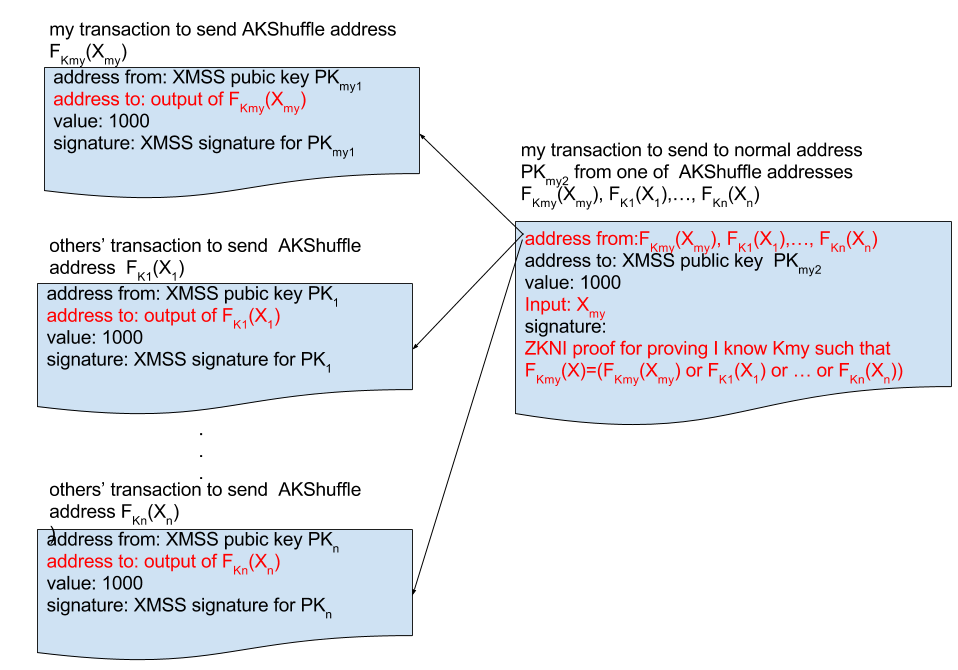
\includegraphics[width=80mm]{shuffle.png}
	  \caption{An example of AKShuffle.}
    \label{fig:shuffle}
	\end{center}
 \end{figure}

 Figure~\ref{fig:shuffle} illustrates transactions related to AKShuffle. One who wants to shuffle her coins sends her coins to a shuffle address.
 The shuffle address is an output of an encryption \( f_{k_{my}}(x_{my}) \) with key \( k_{my} \). 
 \(k_{my}\) is her secret key  and \(x_{my}\) is her public input.
 Some day she wants to  withdraws her shuffled coin. She creates one transaction which sends to her normal address \(PK_{my_2}\) (his XMSS public key).
 The transaction has her AKShuffle address \( f_{k_{my}}(x_{my}) \) with others' AKShuffle addresses 
\( f_{k_{1}}(x_{1}) \), \( f_{k_{2}}(x_{2}) \) \dots \( f_{k_{n}}(x_{n}) \) as input addresses. 
This means nobody knows which address is really used for spending. As signature she fills in ZKNI proof proving she knows \( k_{my} \) such that 
one of AKShuffle addresses in inputs equals  to \( f_{k_{my}}(x_{my}) \). The transaction also includes her public input \( x_{my} \)
to prevent to reuse the shuffle address. Values in transactions must be same.

Notice that transactions for AKShuffle and ones for normal payment are different. AKShuffle (ZKBoo) is used only for shuffling one's coin.
In another word, one cannot use AKShuffle for paying to another.
This is because signature size of ZKBoo is bigger (around 500 KBytes if number of input addresses is 5).


\section{Network}
\label{sec:network}

\begin{figure}[ht]
	\begin{center}
	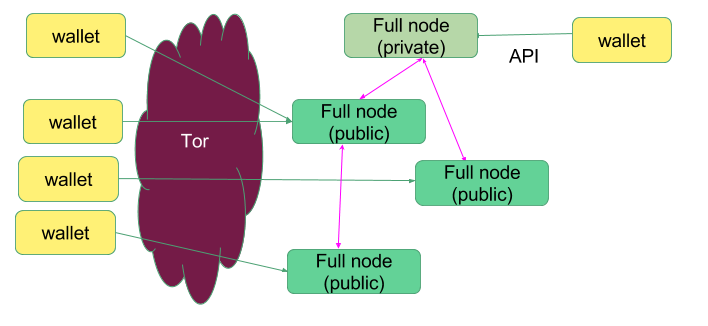
\includegraphics[width=80mm]{network.png}
	  \caption{Full-nodes and clients (wallets) in Aidos Kuneen.}
    \label{fig:network}
	\end{center}
 \end{figure}

 Figure~\ref{fig:network} illustrates network in Aidos Kuneen.
Network for Aidos Kuneen is built with full-nodes in P2P fashion. Clients can connect to these full-nodes
or their own full-nods via API. Clients can send APIs to broadcast their transactions etc, normally by wallet application.
 Between full-nodes transactions are sent and received each other by using some efficient protocol (e.g. msgpack\footnote{https://msgpack.org/})
 to reduce packet sizes. 

We also use Tor for anonymity between public full-nodes and clients. This is because 
full-node can know their clients IP address and what the client sent.  We don't use Tor between full-nodes because efficiency between
full-nodes is critical. Also  there is no way to know who sends the transaction first in network because transactions are relied between 
full-nodes repeatedly.

We would build Kademlia network to use peer discovery scheme in the future for post-quantum anonymity network. 
Unfortunately Tor is not post-quantum, but Tor has big number of participants. We use the benefits of the merit
for strong anonymity for now. But in the future there also many participants in Aidos Kuneen we could build our own anonymous network.
Also we are planning to distribute transactions for more scalability, i.e.\ one full-node don't hold all transactions but can get any certain
transactions from others on network.
We are still investigating for the scheme.

Table~\ref{tbl:cmd} shows commands of packets.

%\clearpage

 \begin{table}[htb]
	\caption{Basic Packet Commands}
    \label{tbl:cmd}
	\begin{tabularx}{\linewidth}{XX} 
		command & description \\
		\toprule
  ping & ping to another node \\
  pong & response of ping \\
  find\_node & request node info\\
    resp\_node & response node infers \\
  req\_transactions & request transactions contents \\
  resp\_transactions & respond transactions contents \\
  req\_leaves & request  leaves' hashes \\
  resp\_leaves &  respond leaves' hashes \\
  invent &  invent a new transaction hash \\
  ack\_invent & ack of invent \\
  invent\_copow & invent that a node is searching for coPoW group \\
  ack\_copow & ack of invent\_coPoW \\
  find\_value &  reserved for future use.\\
  store\_value & reserved for future use.\\
  \bottomrule
\end{tabularx}
  \end{table}


\section{Leaves in iMesh}
\label{sec:leaves}

\begin{figure}[ht]
	\begin{center}
	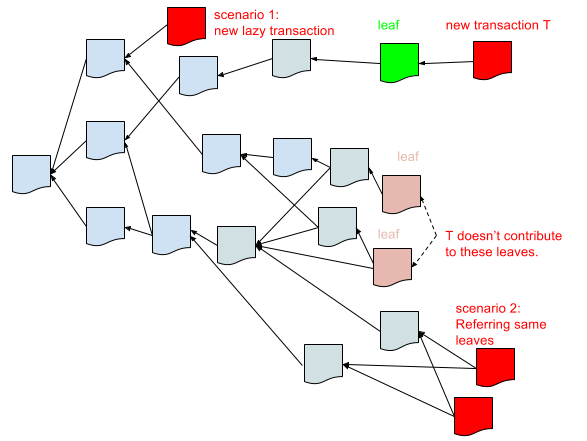
\includegraphics[width=80mm]{leaves.png}
	  \caption{Leaves in iMesh}
    \label{fig:leaves}
	\end{center}
 \end{figure}

As we mentioned in Section~\ref{sec:imesh}, speed of confirmation
depends on the number of leaves \( N_{leaves} \) in iMesh. This is because more leaves exists,
possibility  that one transaction is referred  will be less(Figure~\ref{fig:leaves}).
Some scenarios could make leaves increase.

First scenario is that lazy senders intentionally could refer non-leaves transactions for his transaction.
This adds one leaves without decreasing number of leaves. But the sender is discouraged to be lazy.
As we mentioned confirmation time depends on number of ascendant transactions,
so receiver would refuse its payment if the receiver thinks sender is intentionally lazy.
Second, one transaction \(T_1\) could come into iMesh while another \(T_2\) are doing PoW.
\(T_1\) and \(T_2\) might refer same transactions.
This scenario is not avoidable because it could happen by chance regardless senders' intent.
In third scenario attackers could broadcast many transactions and try to increase enormous leaves to make confirmations slower.
This scenario could be much discouraged by PoW.

To solve second problem,
we could increase number of referring transactions in one transaction \( N_{ref} \) 
to decrease \( N _{leaves} \) (to converge iMesh). But it makes the transaction size bigger.
We want to know the optimal  \( N_{ref} \)  to converge iMesh by modeling the behavior of iMesh.

We assume the process of incoming transactions can be modeled by a Poisson flow, and the time to  complete PoW can be modeled by exponential distribution.
So let \(\lambda_{in}\) the rate of the Poisson flow , and \(1 / \lambda_{pow}\) is the expectation of the time to complete PoW.
Senders make his transaction at rate \(\lambda_{in}\)  and finish PoW in  \(1/\lambda_{pow}\) in average.
This transaction includes referring transactions \( N_{ref}\).
While doing PoW, others might also being making their transaction and might include same transactions.
The fact that  \( N_{ref} (t) \)  depends on  \( N_{ref} (t-t')\) (i.e.\ status in past) makes it difficult 
to solve \( N_{ref}\). Hence we do simulation the behaviour of \( N_{ref}\).

Algorithm~\ref{alg:sim1}  shows the algorithm to simulate number of leaves in iMesh.
We fix  \(1 / \lambda_{pow} = 10 \) minutes (which means PoW has finished in 10 minutes
in average), and simulate with \(N_{ref}\ = 2, 4, 8, 16, 32 \).
And we simulate 4 types of  \(\lambda_{in} \).

\vspace{-0.5\baselineskip}
\begin{enumerate}
	\setlength\itemsep{0em}
\item 1 transaction per minute \\
 This parameter assumes that a few transactions come into iMesh for
early days in iMesh
\item 1 TPS(transaction per second)
\item 5 TPS \\
 This is the maximum rate in Bitcoin occurred in May 2017.
 \item 10 TPS
\end{enumerate}

	\begin{algorithm}[ht]                  
		\caption{Simulation for counting leaves in iMesh}         
		\label{alg:sim1}
		\begin{algorithmic}
			\STATE{INPUT  \(N_{ref}\): number of direct referring transaction}
			\STATE{INPUT \(T_{sim}\): simulation time}
			\STATE{INPUT \(\lambda_{in}\):  process of incoming transactions }
			\STATE{INPUT \(\lambda_{pow}\): period to  complete PoW }
			\STATE{OUTPUT: number of leaves for each time}
			\STATE{}
	\STATE{\(time=0\) //current time}
	\STATE{\(pow\_txs=\{\} \) //transactions which are doing PoW}
	\STATE{\(txs=\{\} \)//transactions in iMesh}
	\WHILE{\(time < T_{sim}\)}
		\STATE{\(step \Leftarrow \)  an exponentially distributed value at rate \(\lambda_{in}\)}
		\STATE{\(time \Leftarrow time + step\)}
	
		\STATE{}
	\STATE{//add a new transaction to the transaction list}
	\STATE{//with a period to finish PoW.}
	\STATE{make new transaction \(t_{new}\)}
	\STATE{\(t_{new}.is\_leaf \Leftarrow true\)}
	\STATE{\(leaves \Leftarrow \) select random \(N_{ref}\) leaves in \(txs\)}
	\STATE{\(t_{new}.leaves \Leftarrow leaves\)}
	\STATE{\(pow\_time \Leftarrow \)  an exponentially distributed value at rate \(\lambda_{pow}\)}
	\STATE{\(t_{new}.pow\_time  \Leftarrow time + pow\_time\)}
	\STATE{append \(t_{new}\) to \(pow\_txs\)}
	
	\STATE{}
	\STATE{//handle transactions whose PoW has finished}
	\FORALL{\(t\) in \(pow\_txs\)}
	\IF{\(t.pow\_time \le time\)}
	\STATE{remove \(t\) from \(pow\_txs\)}
	\STATE{append \(t\) to \(txs\)}
	\FORALL{\(l\) in \(t.leaves\)}
	\STATE{\(l.is\_leaf \Leftarrow false\)}
	\ENDFOR{}
	\ENDIF{}
	\ENDFOR{}
	\STATE{count \(t\) such that \(t.is\_leaf=true\) in \(txs\) and print it}
	\ENDWHILE{}
	\end{algorithmic}
		\end{algorithm}

		Figure~\ref{fig:min1_2} \textasciitilde~\ref{fig:sec10} in Appendix shows the simulation results.
	 The result of \( N_{ref}=8,16,32\) for \( \lambda_{in}=1\) transaction per minute are not shown
	 because these result are much similar to  one of \( N_{ref}=4\).

	 From these results number of leaves \( N_{leaves}\) decreases in an proportional manner following to the number of \( N_{ref} \).
	 Even when  \( \lambda_{in}=1\) transaction per minute, \( N_{ref}=2\) is not enough to converge DAG fully
	 (  \( N_{leaves}\) is around 3 \textasciitilde 26 ),
	 and \( N_{ref} \ge 4\)  is better ( \( N_{leaves}\) = 1 \textasciitilde 18).
	 Further for other \( \lambda_{in}\), \( N_{ref}=2\) is much worse than other \( N_{ref}\).
	 For example at \( \lambda_{in}=5\) TPS,  \( N_{leaves} \simeq 3800 \) when \( N_{ref}=2\),
	\( N_{leaves} \simeq 500\)  when \( N_{ref}=8\). We \emph{should NOT} use \( N_{ref}=2\) if we assume 
	transactions comes into iMesh at same speed as Bitcoin.
	Time to converge DAG is below 3000 seconds (50 minutes) except \( N_{ref}=2\) when \( \lambda_{in}=10\) TPS.
 
	 We also simulate how the number of  transactions \( N_{descendant} \) which refers directly and indirectly to one transaction grows 
	 for each cases above. Figure~\ref{fig:min1_ref} \textasciitilde~\ref{fig:sec10_ref} in Appendix shows the results.
	 
	 In these figures x-axis means the number of transaction which comes into iMesh
	 after iMesh becomes stable. Y-axis means \( N_{descendant} \) 
	 (descendant transactions) of one random transaction. The graph would becomes a diagonal (linear) line if \( N_{descendant} \) grows ideally.
	 When  \( \lambda_{in}=\) 1 transaction per minute,   graphs of all \( N_{ref}\) are almost diagonal.
	 But more  \( \lambda_{in}\) increases,  \( N_{descendant} \) becomes less.
	 For example when  \( \lambda_{in}\) =5 TPS,  \( N_{descendant} \) 
	 doesn't increase diagonally even after  25000 transactions  ( \( 25000 \times 0.2\) seconds \(\simeq 1.39 \) hours in average) at \( N_{ref} \)  = 2.
At \( N_{ref}\) = 8 after  4000 transactions  ( \( 4000 \times 0.2\) seconds \(\simeq 13.3 \) minutes in average),
 \( N_{descendant} \) starts to increase linearly.


	 Our decision is that we make \( N_{ref}\) be variable and
	 for now we set the default to 8. 
	 Even if iMesh grows to  \( \lambda_{in}=5\) TPS, which is the maximum TPS
	 in Bitcoin,  \( N_{ref}=8\) makes iMesh well converge around \#leaves=500. 
	 Also \( N_{ref}=8\)  could
	 help to prevent attackers to increase leaves.
	 They can add at most one leaf per one transaction.  We are assuming attackers have half of the whole hash power, so 
	 of honest transactions refer 8 transactions then 
	 these leaves would be converged very soon.

 	 We could re-view the default number once iMesh will grow higher.

	  \section{Conclusion}
\label{sec:conc}

We presented  a new cryptocurrency \emph{Aidos Kuneen}.
Aidos Kuneen employs \emph{iMesh} where all transactions are directly referred each others and forms  DAG structure.
To prevent  double spendings we utilize `SPECTRE' which determines a legit transaction from DAG structure.
We employ a hash-based signature `XMSS' as a signature scheme for quantum computer resistance.
For anonymity we utilize \emph{AKShuffle} which uses zero-knowledge proof `ZKBoo (ZKB++)` for post-quantum.
For IoTs we introduce cooperative Proof of Work called \emph{coPoW}, by which each senders can do PoW together.
Finally we simulate the number of leaves in iMesh, and look into the behaviour.

Our open problem is the size of transactions. The size is about 3 KBytes for normal transactions and
500 KBytes for AKShuffle transactions. We continue to research better signature schemes and anonymity scheme
for post quantum.

\newpage
\begin{table}[htb]
	\caption{Specification of Aidos Kuneen}
    \label{tbl:spec}
	\begin{tabularx}{\linewidth}{XX} 
		\toprule
		Unit & ADK \\
		\midrule
Total Supply & 25,000,000 ADK \\ 
\midrule
Minimum Unit & 0.00000001 (\(10^{-8})\) ADK \\ 
\midrule
PoW Algorithm & Cuckoo Cycle\\ 
\midrule
Anonymity & AKShuffle (post quantum zero knowledge proof)  and Tor \\
\midrule
Consensus Algorithm & SPECTRE \\ \midrule
Distributed Ledger & iMesh (transaction DAG) \\
\midrule
Signature Scheme & XMSS (post quantum hash based signature)\\ 
\midrule
Usage &  IoT, Finance, Banks, Commerce \\ 
\bottomrule
\end{tabularx}
  \end{table}


  \twocolumn[
	\begin{@twocolumnfalse}

  \begin{thebibliography}{99}
	
	\bibitem{btc}
		Satoshi Nakamoto,
		\emph{Bitcoin: A Peer-to-Peer Electronic Cash System}, 2008.
	
	\bibitem{ietf}
	Crypto Forum Research Group, draft-irtf-cfrg-xmss-hash-based-signatures-10
		\emph{XMSS:Extended Hash-Based Signatures}, 2017.
		
	\bibitem{iota}
	Serguei Popov,
		\emph{The tangle}, 2017.
	
	\bibitem{prob}
	Sheldon M. Ross,
		\emph{Introduction to Probability Models. 10th Edition}, 2012.
	
	\bibitem{dagcoin}
	Sergio Demian Lerner,
		\emph{DagCoin: a cryptocurrency without blocks}, 2015.
	
	\bibitem{xmss}
	Johannes Buchmann, Erik Dahmen, Andreas H\"ulsing,
		\emph{XMSS --- A Practical Forward Secure Signature Scheme Based on Minimal Security Assumptions}, 2011.
	
	\bibitem{zkboo}
	Irene Giacomelli, Jesper Madsen, Claudio Orland,
		\emph{ZKBoo: Faster Zero-Knowledge for Boolean Circuits}, 2016.
		
	\bibitem{zkb}
	Melissa Chase, David Derler, Steven Goldfeder, Claudio Orlandi, Sebastian Ramacher, Christian Rechberger, Daniel Slamanig, Greg Zaverucha,
		\emph{Post-Quantum Zero-Knowledge and Signatures from Symmetric-Key Primitives}, 2017.
		
	\bibitem{spectre}
	Yonatan Sompolinsky, Yoad Lewenberg, and Aviv Zohar, 
		\emph{SPECTRE:	Serialization of Proof-of-work Events: Confirming Transactions via Recursive Elections}, 2016.
	
	\bibitem{shor}
	Peter W. Shor, 
		\emph{Polynomial-Time Algorithms for Prime Factorization and Discrete Logarithms on a Quantum Computer}, 1995.
		
	\bibitem{google}
	Masoud Mohseni, Peter Read, Hartmut Neven,
		\emph{Commercialize early quantum technologies}, 2017.
		
	\bibitem{recom}
	PQCRYPTO,
		\emph{Post-Quantum Cryptography for Long-Term Security, Initial recommendations of long-term secure post-quantum
		systems}, 2015.
			
	\bibitem{ringsig}
	Nicolas van Saberhagen,
		\emph{CryptoNote v 2.0}, 2013.

	\bibitem{cuckoo}
	John Tromp,
		\emph{Cuckoo Cycle: a memory bound graph-theoretic proof-of-work}, 2014.

	\bibitem{byteball}
	Anton Churyumov,
		\emph{Byteball: A Decentralized System for Storage and 	Transfer of Value}.	

	\bibitem{traverse}
	Michael Szydlo,
		\emph{Merkle Tree Traversal in Log Space and Time}, 2004.	

	\end{thebibliography}
	
	\end{@twocolumnfalse}
	]


\clearpage

\appendix
\section{Results of Simulation}
\label{ap1}

\begin{figure}[ht]
	\begin{center}
	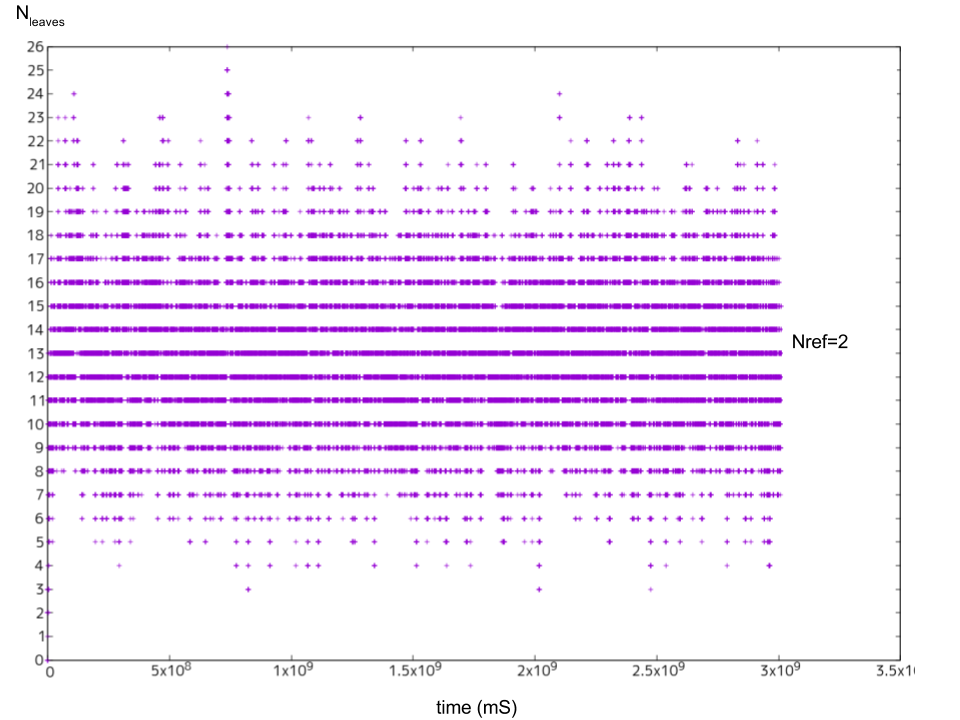
\includegraphics[width=80mm]{1min_2.png}
	  \caption{Number of leaves at \( \lambda_{in}=\) 1 transaction per minute, \( N_{ref}=2\)}
	\label{fig:min1_2}
	\end{center}
 \end{figure}

 \begin{figure}[ht]
	\begin{center}
		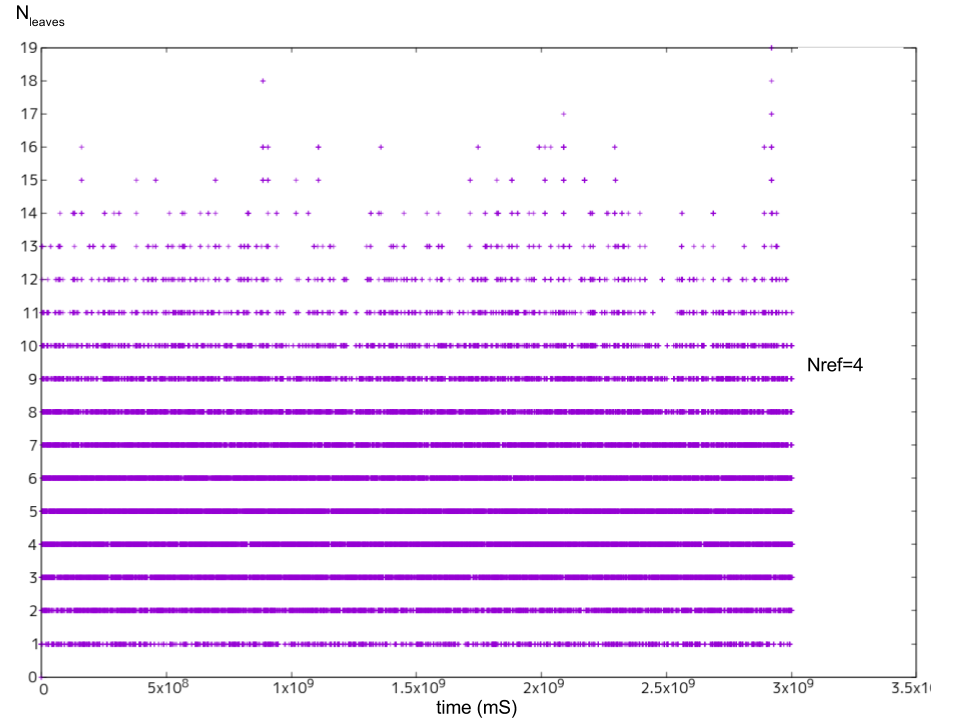
\includegraphics[width=80mm]{1min_4.png}
		\caption{Number of leaves at \( \lambda_{in}=\) 1 transaction per minute, \( N_{ref}=4\)}
	  \label{fig:min1_4}
	\end{center}
 \end{figure}

 \begin{figure}[ht]
	\begin{center}
	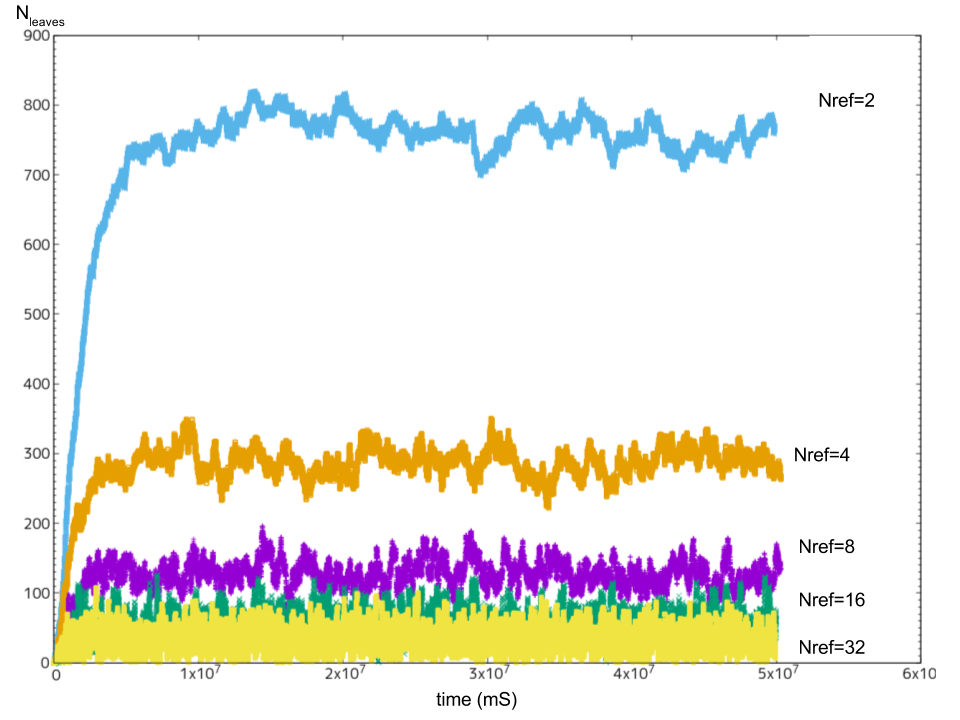
\includegraphics[width=80mm]{1sec.png}
	  \caption{Number of leaves at \( \lambda_{in}=\) 1 TPS}
	\label{fig:sec1}
	\end{center}
 \end{figure}

 \begin{figure}[ht]
	\begin{center}
	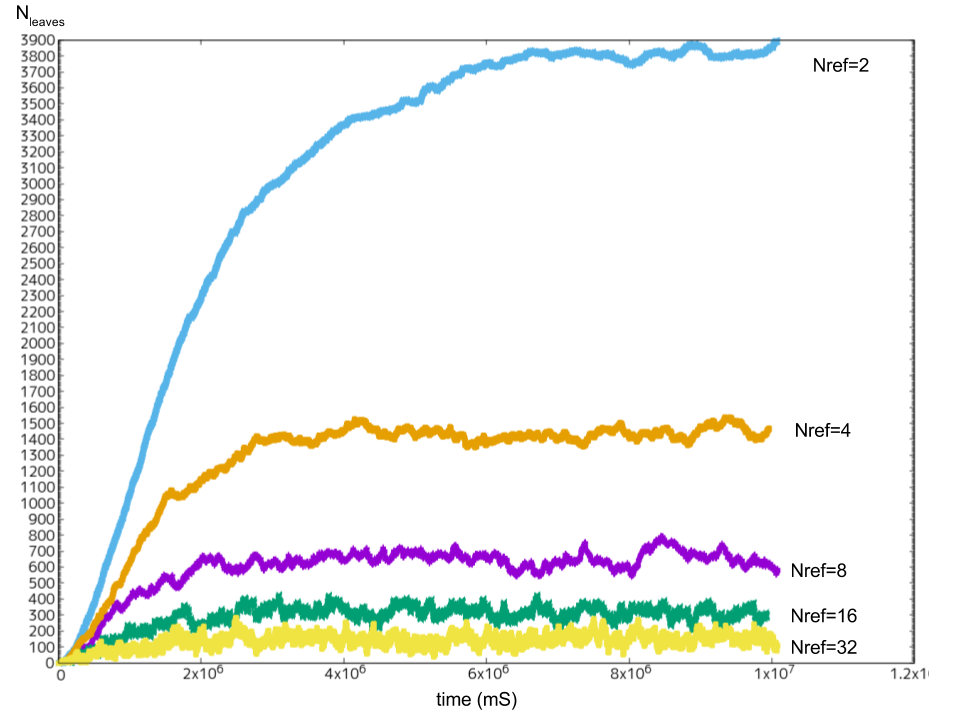
\includegraphics[width=80mm]{5sec.png}
	  \caption{Number of leaves at \( \lambda_{in}=\) 5 TPS}
	\label{fig:sec5}
	\end{center}
 \end{figure}

 \begin{figure}[ht]
	\begin{center}
	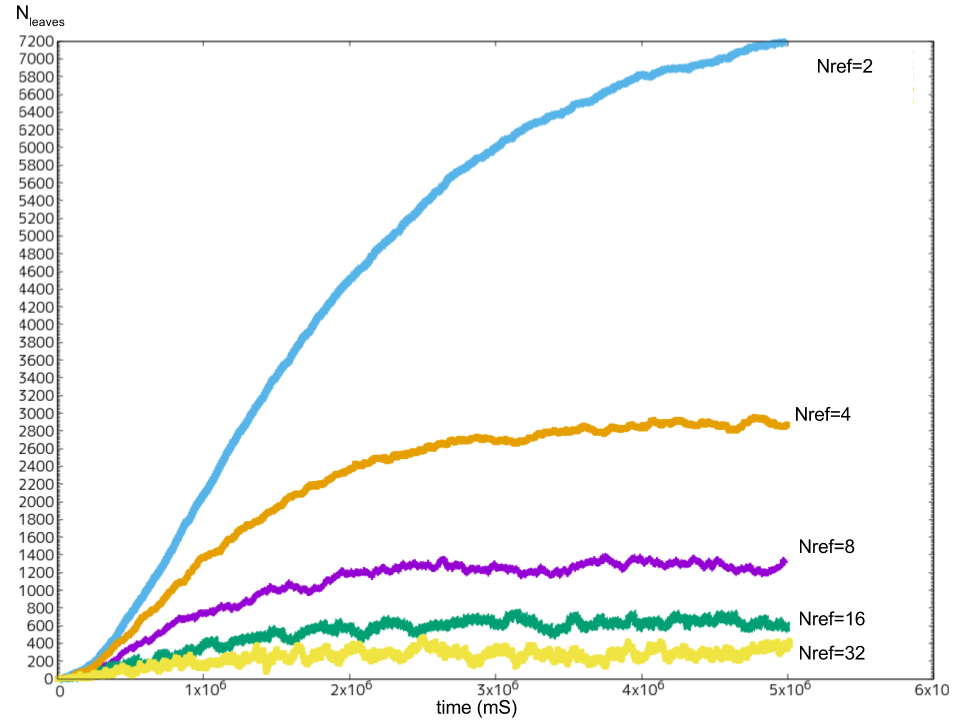
\includegraphics[width=80mm]{10sec.png}
	  \caption{Number of leaves at \( \lambda_{in}=\) 10 TPS}
	\label{fig:sec10}
	\end{center}
 \end{figure}

 \begin{figure}[ht]
	\begin{center}
		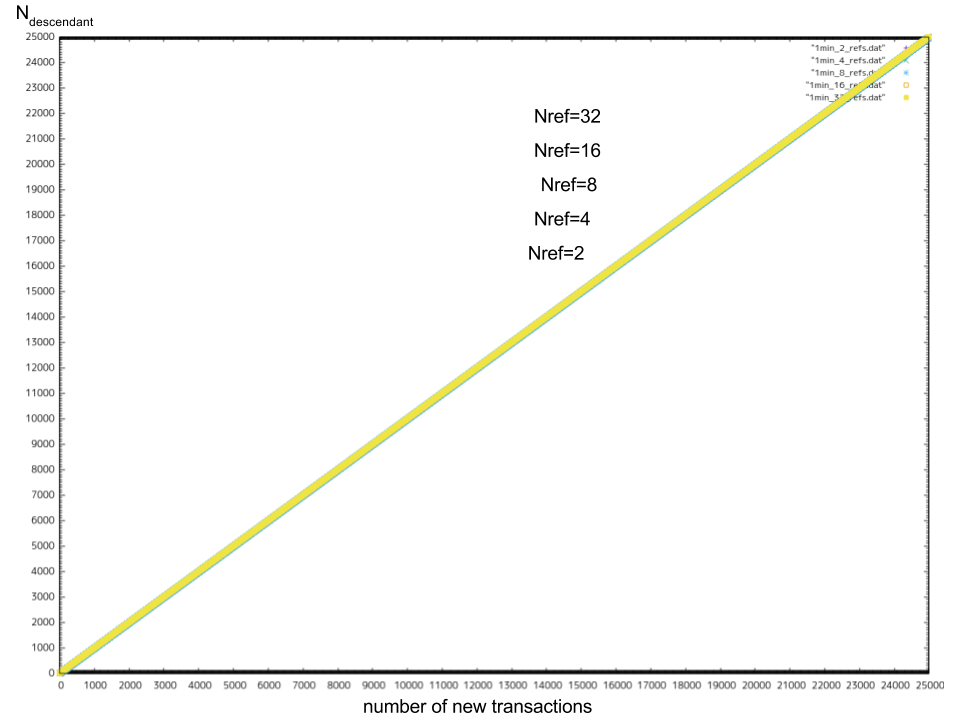
\includegraphics[width=80mm]{1min_ref.png}
		\caption{Growth of \(N_{descendant}\) at \( \lambda_{in}=\) 1 transaction per minute}
	  \label{fig:min1_ref}
	\end{center}
 \end{figure}

 \begin{figure}[ht]
	\begin{center}
		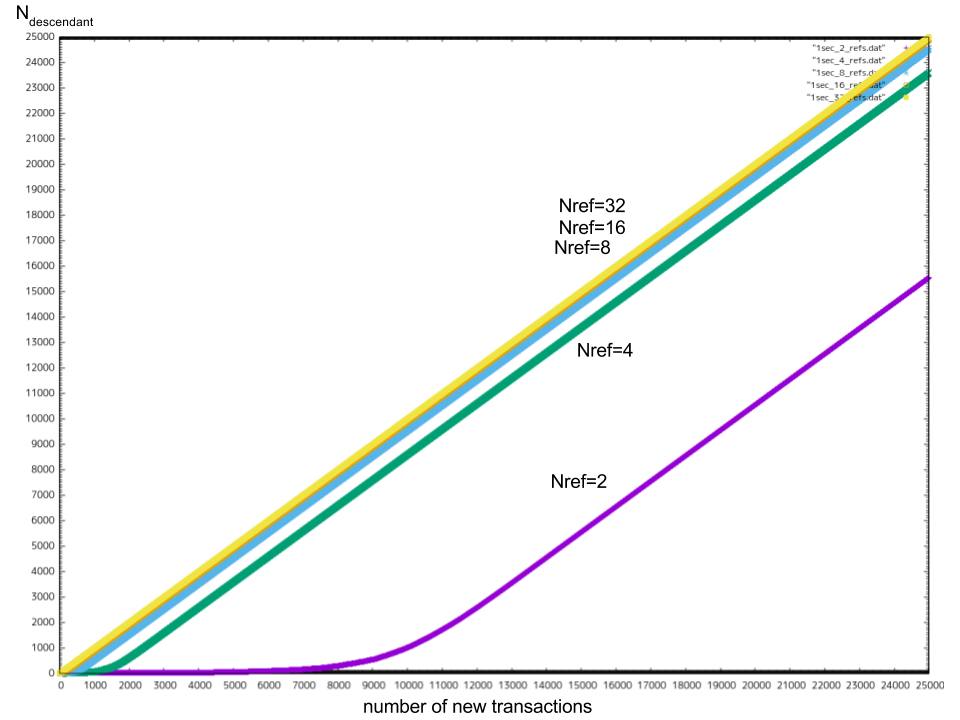
\includegraphics[width=80mm]{1sec_ref.png}
		\caption{Growth of \(N_{descendant}\)  at \( \lambda_{in}=\) 1 TPS}
	  \label{fig:sec1_ref}
	\end{center}
 \end{figure}


 \begin{figure}[ht]
	\begin{center}
		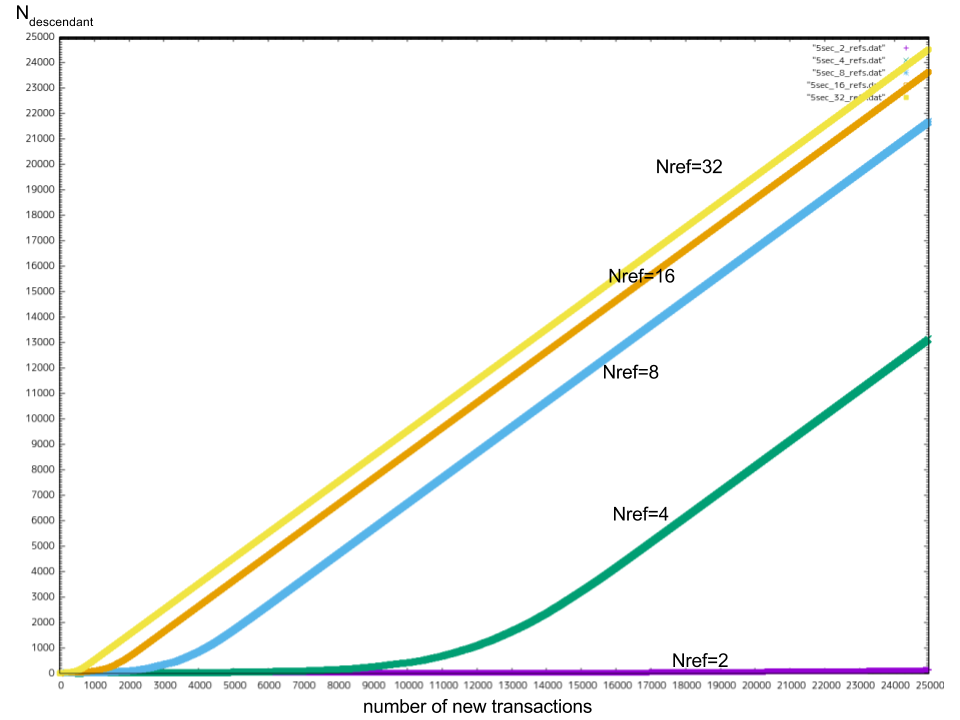
\includegraphics[width=80mm]{5sec_ref.png}
		\caption{Growth of \(N_{descendant}\)  at \( \lambda_{in}=\) 5  TPS}
	  \label{fig:sec5_ref}
	\end{center}
 \end{figure}

 \begin{figure}[ht]
	\begin{center}
		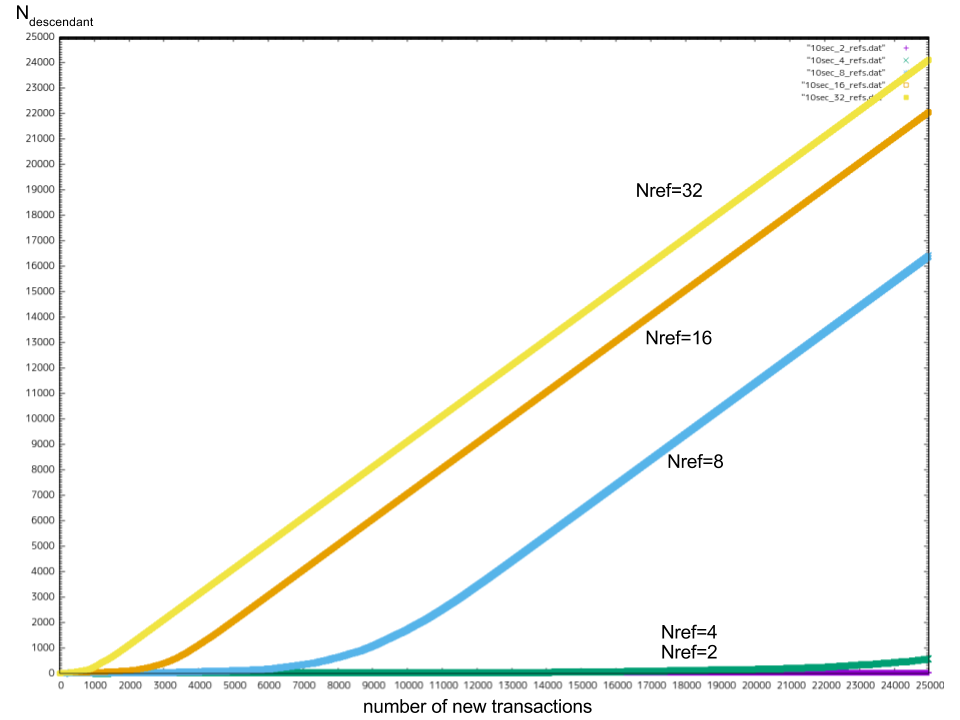
\includegraphics[width=80mm]{10sec_ref.png}
		\caption{Growth of \(N_{descendant}\) at \( \lambda_{in}=\) 10 TPS}
	  \label{fig:sec10_ref}
	\end{center}
 \end{figure}
 
 
  
\end{document}
